% ============================================
% First column, Introduction
% ============================================

\separatorcolumn

\begin{column}{\colwidth}

    \begin{exampleblock}{Environments in nuclear systems}

        \heading{Ten percent of the world electricity is produced \textit{via} nuclear reactors, in which structural components are exposed to an aggressive and complex environment over decades.}

        \begin{itemize}
            \setlength\itemsep{1em}
            \item Neutron radiation leads to atomic displacement / defects / dislocations.
            \item High temperature (\qty{\approx 350}{\degreeCelsius}) and high coolant pressure (\unit{\mega\pascal}).
            \item Mechanical stress, vibrations.
            \item Corrosive aqueous environment, radiolysis product / nuclear reactivity controlled with additives.
            \item \textbf{Effects can take between minutes and years to manifest.}
        \end{itemize}

    \end{exampleblock}

    \begin{block}{Radiation damage, corrosion and embrittlement}

        \begin{figure}
            \centering
            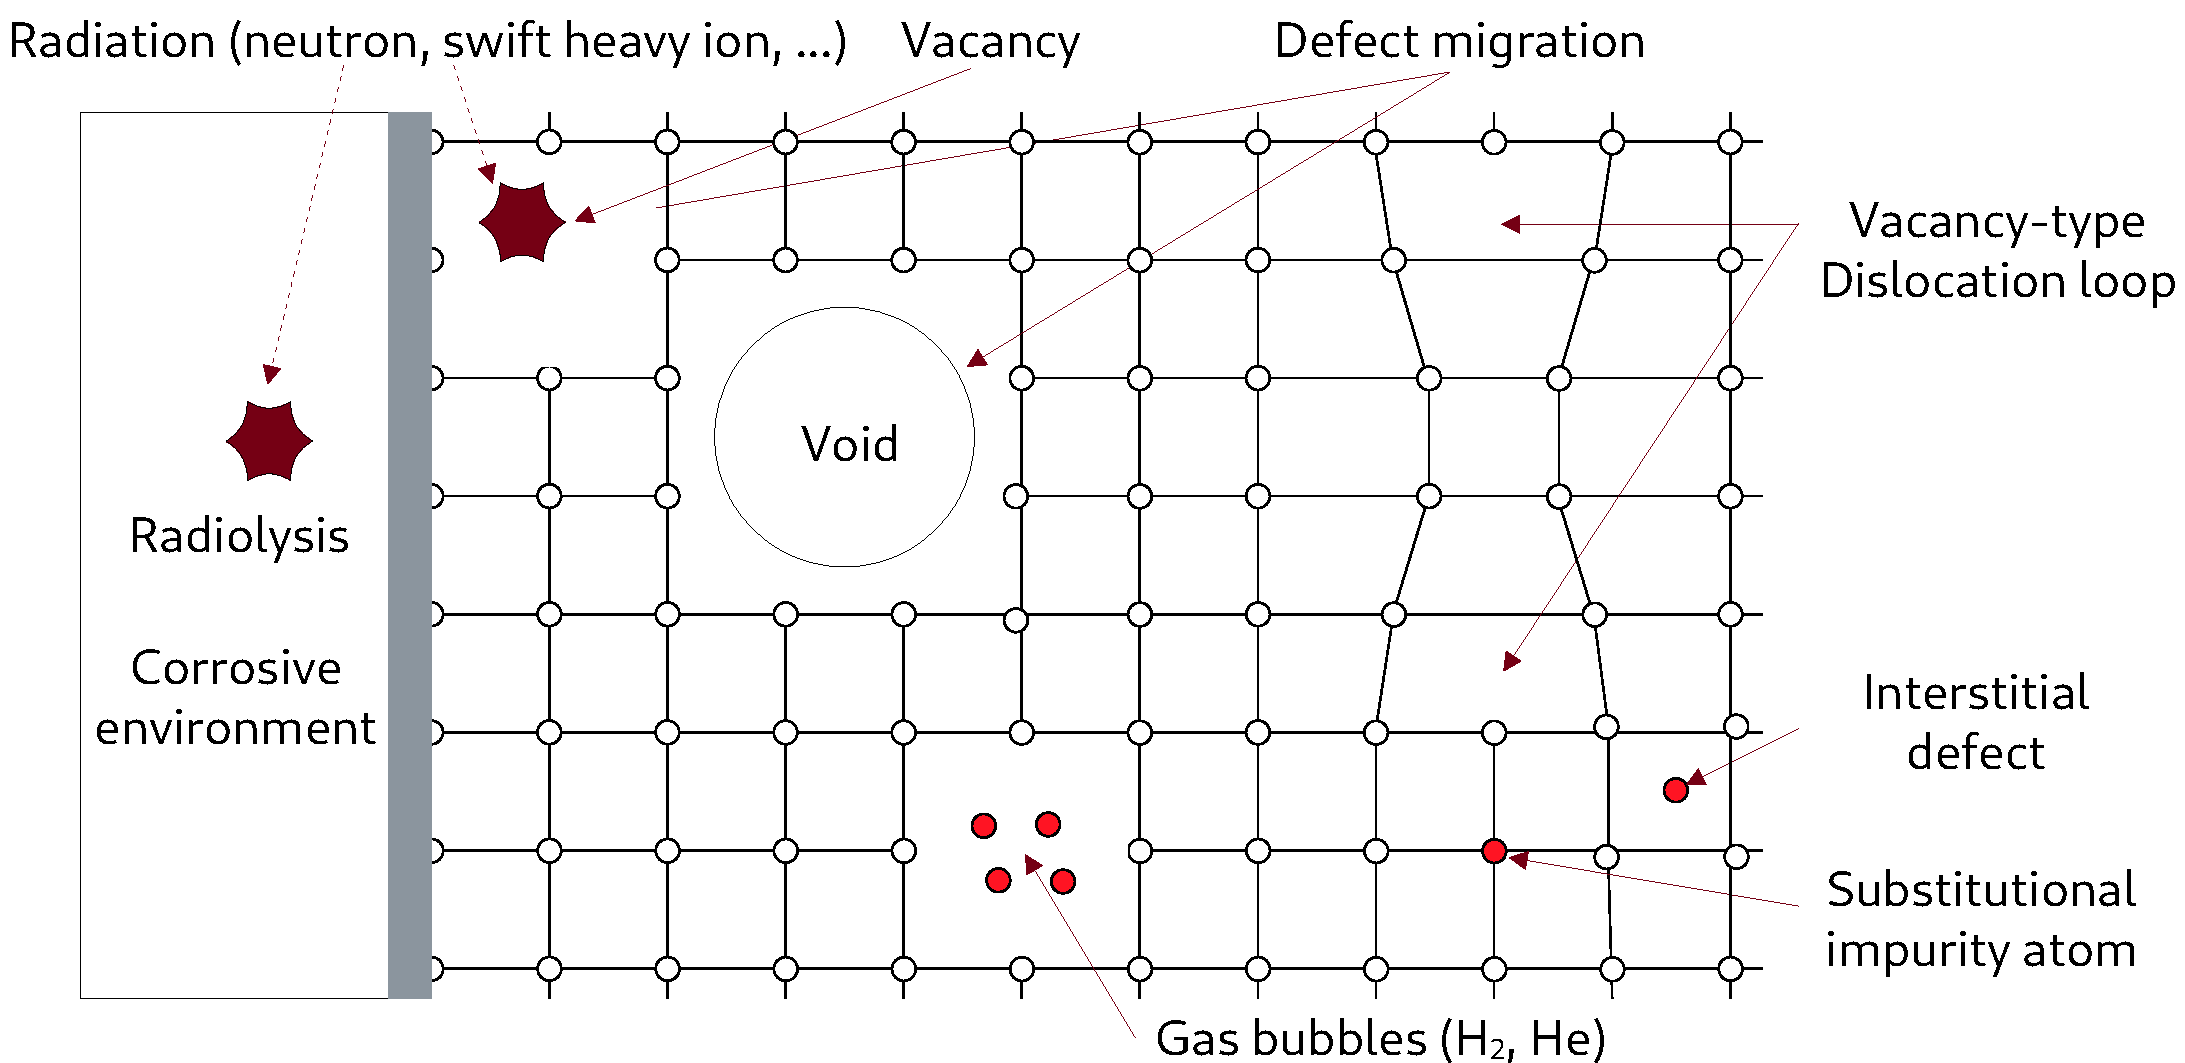
\includegraphics[width=\colwidth]{IntroductionMIT/RadiationDefects.pdf}
            \caption{Neutrons can displace atoms, creating a variety of defects.}
            \label{fig:DefectsLattice}
        \end{figure}

    \end{block}

    \begin{block}{Which materials are present?}

        \begin{columns}[T]
            \begin{column}{0.5\colwidth}

                \heading{Large variety of alloys.}

                \begin{itemize}
                    \setlength\itemsep{1em}
                    \item Pressure vessel: ferritic steel.
                    \item Corrosion resistant passivating layer: Ni-based alloys, Ni-Fe-Cr alloys, stainless steels.
                    \item Fuel cladding: zirconia alloys.
                \end{itemize}

            \end{column}

            \begin{column}{0.5\colwidth}

                \begin{figure}
                   \centering
                   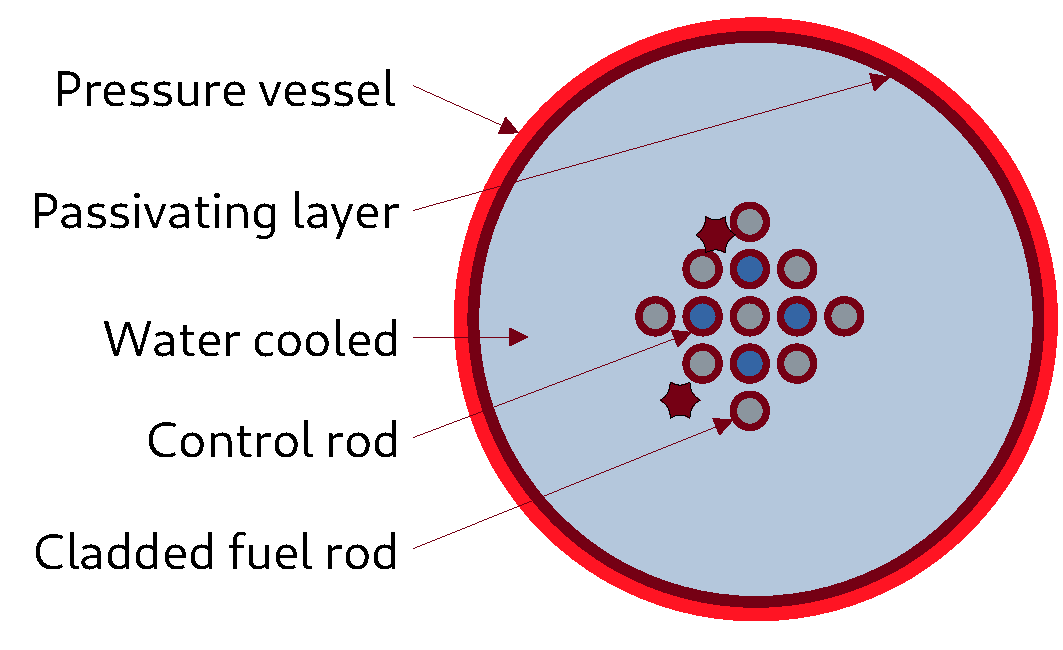
\includegraphics[width=0.49\colwidth]{IntroductionMIT/Vessel.pdf}
                   \caption{Light water reactor schematic.}
                   \label{fig:LWR}
                \end{figure}

            \end{column}
        \end{columns}

    \end{block}

    \begin{block}{Defect control}

        \heading{Heavy ion irradiation can reproduce neutron irradiation effects.}

        \begin{itemize}
            \setlength\itemsep{1em}
            \item Before / after irradiation.
            \item Ion of different nature -> interstitial defects.
            \item Ion nature, fluence and energy \rightarrow damage depth profile.
            \item We have a nuclear reactor \& an ion accelerator.
        \end{itemize}

        \begin{figure}
            \centering
            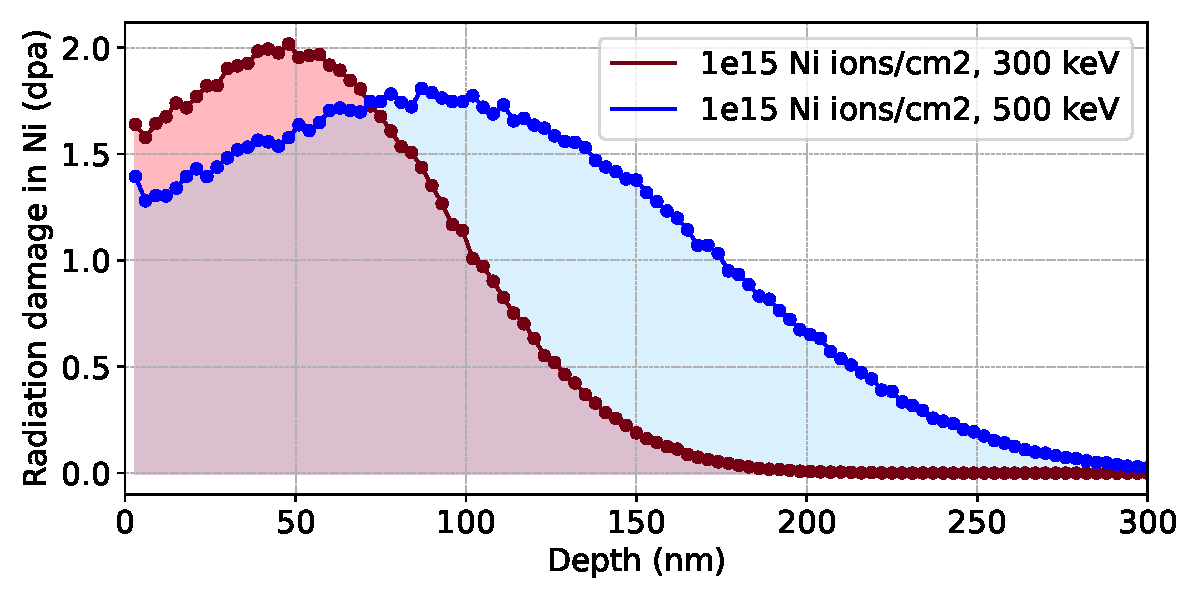
\includegraphics[width=\colwidth, trim=0 10 0 5, clip]{Radiation/NiSingleCrystals/Figures/500keV_and_300keV_DPA_damage_transfer.pdf}
            \caption{Ni ion radiation damage profile, computed with SRIM.}
            \label{fig:NiIonDamage}
        \end{figure}

        \heading{Nano-indentation allows dislocation studies.}

        \begin{itemize}
            \setlength\itemsep{1em}
            \item Before / after dislocation introduction.
            \item Dislocation type, role and mobility characterisation.
        \end{itemize}

    \end{block}

    \begin{alertblock}{Synchrotron radiation for \textit{operando} studies}

        \centering
        \begin{enumerate}
            \setlength\itemsep{1em}
            \item How does neutron radiation affect structural materials?
            \item How to measure the material's structural evolution in a \textbf{relevant} coupled environment?
            % \item Can we use radiation to stabilise some systems?
        \end{enumerate}

        \bigskip
        Standard imaging techniques do not yet offer a combined access to \textbf{operando} and \textbf{high resolution} setups.

        \bigskip
        Synchrotron radiation provides intense, coherent, focused, and tunable X-rays that allow us to work in complex environments!

    \end{alertblock}

\end{column}
